% Preamble
% ---
\documentclass{article}

% Packages
% ---
\usepackage{amsmath} % Advanced math typesetting
\usepackage[utf8]{inputenc} % Unicode support (Umlauts etc.)
\usepackage[english, ngerman]{babel} % Change hyphenation rules
\usepackage{hyperref} % Add a link to your document
\usepackage{graphicx} % Add pictures to your document
\usepackage{listings} % Source code formatting and highlighting
\usepackage{csquotes}
\usepackage{makecell}
\usepackage{multirow}
\usepackage{diagbox}
\usepackage{booktabs, tabularx}
\usepackage{parskip}
\usepackage[backend=bibtex,style=verbose-trad2]{biblatex} % Use biblatex package
\bibliography{quick} % The name of the .bib file (name without .bib)
\usepackage{abstract}
\setlength{\absleftindent}{0mm}
\setlength{\absrightindent}{0mm}
\setlength{\parindent}{0mm}


% Main document
% ---

\begin{document}
\selectlanguage{english}
% Set up the maketitle command
\author{Georges Leschener M. Essomba}
\title{Taxonomy of Microservices}
\date{18th August 2019} % You can remove \today{} and type a date manually

\maketitle{} % Generates title

\pagebreak % Start new page.
\tableofcontents % Generates table of contents from sections
\pagebreak % Start new page

\renewcommand*\abstractname{\flushleft\textbf{Abstract}\hfill}
\begin{abstract}

\noindent Microservices are a relatively new paradigm for building applications. This new paradigm uses an architectural design style for building applications in a loosely coupled components. One of the advantages introduced by such design approach is the ease of maintenance and the ability to change fast. The benefits that microservices bring about have made them very popular and as a result a variety of (open source and proprietary) microservices made available is increasing by the day. This also poses a challenge regarding the complexity of designing applications from microservices. While the number of microservices publicly available seems to be growing exponentially, a good number of them are just a replication of other ones. This raises the issue of duplication of effort from engineers who invest time in building microservices which in some cases already exist instead leveraging common building blocks and patterns and only add capabilities that are unique to each microservice. This paper defines a taxonomy for microservices by looking into public repositories of microservices and identify common patterns in their design, use cases and interoperability. We look at how microservices could be classified enabling those with an interest in acquiring microservices to select the right microservice when in need (say when building an application) based on a pattern fits best their use cases (functional fit) and or certain technical characteristics (technology fit) that are specific to their environment. One of the usages of this taxonomy might be the design of a discovery mechanism for the automated discovery of microservices which is beyond the scope of this study.


\end{abstract}


\section{Introduction}


Garriga (2018) defines Microservices as a novel architectural style that overcomes the shortcomings of centralized, monolithic architectures, in which application logic is encapsulated in big deployable chunks. In contrast, microservices are small components, built around business capabilities, that are easy to understand, deploy, and scale independently, even using different technology stacks. Each microservice runs in a dedicated process and communicates through lightweight mechanisms, often a RESTful API.


Namiot \& Sneps-Sneppe (2014) introduce the microservices approach as a relatively new term in software architecture patterns which consists in developing an application as a set of small independent services with each service running in its own independent process. Five years have passed since the introduction of microservices. Today, the fact of the matter is that the adoption of microservices is growing at a rapid pace as many businesses are looking to move away from legacy architecture design style. Monilith applications which is one such legacy approach as remark Singleton (2016) are known to significantly slowdown application development lifecycle and lead to very risky and costly maintenance and upgrades. With microservices instead, businesses take advantage of new computing paradigms such as cloud computing, DevOps, Continuous integration, continuous delivery (CI/CD) to name but a few.


There are many definitions of microservices that have been given by many researchers and they all seem to convey a common view of the attributes of microservices which include “loosely coupled”, “independently developed, deployed and maintained”, “using lightweight communication”, “small in size”. According to Chen (2018) microservices enable teams to produce software reliably in short release cycles and at any time. The downsides of that however is that it could lead to duplicate efforts as different teams or independent software developers may end up building the same microservices or components that fulfill the same functionality leading to wasted time, and resources.


While such an approach would offer a plethora of options to designing applications or services from loosely coupled components (microservices) and as such provide more options in terms of the business functionalities that could be fulfilled by those applications or services. It also makes it very complex and time-consuming task to assemble a particular end product or service capable of fulfilling a given function. That is precisely why Chen (2018) was quick to remind us while presenting the benefits of microservices that they are not silver bullet as their adoption does introduce complexities and challenges which, if not managed properly could lead to another problematic situation. One of the challenges is today microservice discovery and composition based on a set characteristics. Such a functionality would require a common repository for storing and publishing microservices and a well-defined framework for classifying them. That way one could easily discover microservices that provide common functionalities as well the one specifically designed to fulfill a specific function. The added value of such framework is that it would help eliminate duplicate effort and reduce time and cost of building microservice-based applications. Automated discovery of microservices would mean having a taxonomy for understanding, grouping and classifying microservices based on common attributes. it does also present a number of challenges associated with microservices notably two of them which are the challenge related with searching for a particular type of microservice and where exactly to search for it. For the former this could be addressed by way of a rigorously designed taxonomy to help identify common patterns or attributes that microservices share which could be used for their classification and this is precisely what we attempt to do in this research.

Soldani et al. (2018) study on the pains and gains of microservices while it does provide good pointers in terms of the challenges and benefits that are to be expected by microservices adopters. This is particularly valuable for the challenges in that it helps those planning to adopt microservices be aware of the risks they could potentially encounter which means they could put in place strategies to proactively mitigate those risks. As such Soldani et al. (2018) taxonomy which is not intended to help with the classification of microservices does not overlap in any way with our taxonomy. 

That being said, there are some similarities in Garriga’s taxonomy with ours as both encompass technical aspects of microservices. Equally there are some significant differences between the two taxonomies as already mentioned. The newly proposed taxonomy provides another dimension through which microservices could be classified, which has the advantage of addressing the needs on microservices classification for both a technical and non-technical audience is one of the main motivations for this study. Looking at microservices from a perspective of the functionalities they are intended to fulfil and combining that with non-functional characteristics should complement very well the work done by Garriga (2018). Newman (2015) explains that microservices are primarily modelled around business domains - say microservices providing monitoring or logging functionalities - which helps avoid problems related to traditional tiered architectures. This paper aims to produce a taxonomy for microservices to help with their classification in a fine-grainer way that would account for both functional and non-functional attributes of microservices. For testing the taxonomy, we use an example of microservice taken randomly from Amazon Serverless architecture repository \url{https://serverlessrepo.aws.amazon.com/applications} which is Amazon Web Services repository for microservices which is open to the public and free of charge. 

This paper is organized as follows: in the section 2 we will look into related work, in section 3 we explain the need for this new taxonomy and the target audience, then in section 4 we define our research questions followed the methodology in section 5, and in section 6 and 7 we describe the new taxonomy explaining how it helps answer the research questions, and in section 8 we go over an example of classifying microservices using our taxonomy. In section 9 we present the limitations of our methodology before concluding and looking at opportunities for further research in section 10.



\section{Related work}


A quick search on google scholar on microservices taxonomy return a number of results for which the most significant are the work done by Garriga (2018) who already had done some similar work classifying web services in the context of Service Oriented Architecture (SOA). For their work on microservices taxonomy, the researcher basically based his study on 64 relevant articles on microservices which he found from searching popular online libraries including Scopus, Science Direct, IEEE Xplore, ACM Digital Library, SpringerLink, Google Scholar and Wiley Online. He then conducted a detailed qualitative analysis on those 64 articles which reduced the list down to 46 articles which he basically classified into two main groups: primary studies, that is, literature investigating specifically their research question (using microservices, proposing microservice-oriented frameworks, tools or architectures) and 28 out the 46 articles were marked as being part of that group; and secondary studies for the remaining 18, that is, literature reviewing primary studies (surveys, reviews and comparative studies assessing microservices or microservice-based approaches). He classified microservices based on 6 dimensions including design, implementation, deployment, runtime, crosscutting concerns and organizational aspects which they further classify into 18 sub-dimensions. Vural et al. (2017) identify 8 characteristics for microservices including: 1. componentization via Services, 2. organized around Business Capabilities, 3. products not Projects, 4. smart endpoints and dumb pipes, 5. Decentralized Governance, 6. decentralized Data Management, 7. infrastructure Automation, 8. design for failure. Those characteristics overlap with Garriga’s classification for instance the design and infrastructure management. Garriga (2018) notes that there is still limited academic efforts in the design patterns and practice for microservices despite the heavy business push towards what he calls “microservitization”. According to the researcher, it is essential to find the right balance between the size and the number of microservices to be able to unlock the potential for the more microservices in the architecture the more business functionalities that they support but this adds more complexity on the network communication and distribution level. From an implementation standpoint, the researcher reckons that microservices are mostly built using lightweight, scripting languages such as JavaScript or Python. Microservices need to interact with one another either as part of single application or as part or interaction between two or more applications and Garriga (2018) interestingly through his study reveals that synchronous interaction mode appears to be the most widely used model as opposed to asynchronous communication even though he reckons that the latter is the most suitable of the two for microservices given that microservices bring decentralization, performance and fault tolerance. Alshuqayran et al. (2016) remarks that deployment is one of the most important and highly discussed topics on microservices as is performance. Taibi (2018) argue that deployment of microservices are still unclear particularly for the ones that are deployed on a private virtual machine which requires a complete start-up. This limits the possibility of a quick deployment while adding to the overhead of maintainability with all VM maintenance, OS, or service container related tasks that need to be done on the machine.  In terms of data exchange, RESTful HTTP communication is the defacto standard for implementing microservices as noted by Garriga (2018) who also cites in his study the efforts to standardize RESTful API through the OpenAPI specification. Considering that one of the issues related to microservices that is often mentioned is the lack of standards with each developer not really having to obey any form standards for building microservices other than the rules of the underlying technologies such as the programming languages or networking protocols. Baresi et al. (2017) proposed an approach for the identification of microservices that consists in matching some of the semantics used in the OpenAPI specifications against a reference vocabulary. This process is known as DISCO-based semantic assessment algorithm or simply decomposition algorithm. Garriga (2018) also remarks that relational databases are still the choice of data store for microservices despite the growing popularity of NoSQL databases while public cloud appears to be the preferred deployment platform for microservices. Similarly, their study showed that microservices are perfectly designed to work with containers though virtual machines were presented as a popular runtime alternative. Sun et al. (2015) cited in Garriga (2018) discuss the security vulnerability of microservices which according to them are designed to trust each other, a feature that could be exploited by malicious users with the possibility to bringing down an entire application. From crosscutting concerns standpoint Garriga (2018) note that microservices in general would have availability and resiliency capabilities incorporated into them citing some examples like circuit breaker and bullhead and from maintainability perspective, the researcher suggests that further study to be done to understand how standards and good practices with automate the maintainability of microservices. Still according to the study from Garriga (2018), DevOps is presented as key aspect for the successful adoption of microservices.

\section{The need for a new taxonomy and intended audience}

Soldani et al. (2018) work on microservices focus on their pains and gains and introduce another taxonomy for the pains of microservices. It is basically a 3-stage taxonomy with each stage known to have specific concerns and pains. The stages align with common steps of software development lifecycle. The first one is the design stage for which the main concern is architecture security with some of the pains identified as API versioning, CI/CD, Access control, etc. The second stage is the development stage whose main concerns are microservices, storage and testing with the biggest pains being around microservices separation, data consistency, integration testing, performance testing, distributed transactions. The third stage is operations which is meant to deal with management, monitoring and resource consumption concerns and the pains identified by Soldani et al. (2018) for this stage are service coordination, logging, cascading failure, compute and network issues. The researchers then conducted a systematic review of 51 industrial studies which showed that the biggest concern for microservices are their architectures, the distributed and heterogeneous storage which renders rather complex the work of developers. Management and monitoring of microservices also appear to be major concern for every industrial study. Soldani et al. (2018) also find out that “security, testing and resource consumption are also notable concerns, while the concrete development of each microservice is not significantly perceived as problematic”. While Tetiana \& Anya (2018) study discuss a taxonomy of microservices security which they basically see as a 6-layered model suggesting that microservices would be best secured at the hardware layer say by using hardware security modules (HSM), virtualization layer, cloud, communication layer, service/application and orchestration. It is clear on reviewing related work that none of the proposed taxonomy look at microservices from a functional prism and as such would not be able to help a practitioner in their selection process of the best technologies for building microservices based on the function or user's requirements that they are designed to fulfill. Likewise academia that have interest in conducting business-related research on microservices would be interested in the classification of microservices from functional perspective and what types of technology would be the best fit for building a particular type or functional microservices.


In the next section we discuss the methodology used for our study to help the reader understand how we arrived into the conclusion of our study, that is the design of a new taxonomy for microservices.

\section{Research questions}

Previous work done by other researchers as discussed already provide a great foundation for understanding microservices. The taxonomy produced by Garriga (2018) in particular is based exclusively on technical or non-functional aspects related to microservices. And while it covers all key stages of the entire lifecycle of microservices helping effectively understand, assess and select microservices based approaches, it does not however look at microservices from a non-technical or functional prism. In order to close that gap we try to answer the following research questions:

\textit{\textbf{RQ1:} What are the functional (non-technical) attributes of microservices?} The taxonomy developed by Garriga (2018) classify microservices based on their technical attributes ignoring the equally important functional characteristics. Though it could be argued the aim of Garriga's work was not specifically to help with the classification of microservices but rather to enable their understanding from their entire lifecycle. Nevertheless, it is still a good foundation that this research will build upon, and answering this research question will hopefully help to expand on such related work. 

\textit{\textbf{RQ2:} How do functional attributes of microservices relate to technical ones?} This question would help to establish whether certain functional attributes map to specific technical attributes of microservices. This ultimately would help understand whether requirements for a microservice-based application or service from a given user have the highest probability of being fulfilled optimally when microservices used to design the application have specific technical attributes

\textit{\textbf{RQ3:} How to classify, select microservices on the basis of the business functionalities they are designed to fulfilled?} Building on the responses to the other two research questions, this one aims to establish whether it is possible to classify microservices on the basis of their attributes both technical and non technical as well as providing a way to guiding practitionners to make optimal selection of technology to build microservices that best meet their requirements.

Answering the above research questions would help create a taxonomy of microservices that would be of interest to practitioner and in particular a non-technical audience. Similarly, scholars or business leaders who have little or no technical knowledge about microservices but who are involved in the decision-making process of microservices adoption in their organization would hardly find answers to their questions on non-technical aspects of microservices from a rather technically-focused study.

\section{Methodology}


To devise our taxonomy, we relied on two sets on data: 1) we searched for primary studies based on microservices taxonomy keywords, 2) we searched repositories of microservices and then we applied each set separately a number of exclusion and inclusion criteria iteratively until we obtained a final list of results. The first set of data formed the basis of our literature review while the second was used to design our taxonomy. The criteria by which microservices were selected or excluded in this study are explained in the next section in order to enable readers to understand why some microservices were selected while other ones were excluded. This process was undertaken according to the prescription of Systematic literature review (Keele, 2007) which recommends devising a well-defined search strategy.


\subsection{Search strategy}


We used the following search strings to identify existing primary studies that relate to microservices taxonomy. We also searched for any systematic literature review on microservices both of which formed the basis of our literature review:


(“taxonomy” OR “classification” OR “characteristics” “properties” OR “systematic literature review”) AND (“microservice” OR “micro-service)


\begin{itemize}
\item Google Scholar
\item University of Leicester online library
\item IEEE Xplore
\item ACM Digital
\item SpringerLink
\item Wiley Online
\end{itemize}

\subsection{Selection of primary studies to include in the review}

The initial search results were evaluated according to clearly defined inclusion and exclusion criteria and through several iterations we were able to reduce the initial 1200 papers to only 20.

The following inclusion-exclusion criteria were applied:

\subsubsection{Microservices primary studies search inclusion criteria}

\begin{enumerate} 


\item All papers that returned from our search criteria
\item Criteria 1 above + date of publication: 2016 or later
\end{enumerate}

\subsubsection{Exclusion criteria}


\begin{enumerate}


\item Any paper that did not contain at least any two of the combined keywords with AND operator. For examples “microservices” AND “taxonomy”
\item Any paper that contains the keywords but its research does not really focus on microservices 
\end{enumerate} 

The diagram shown in figure 1 below depicts the different steps undertaken as part of the search strategy for this study. We basically started by running a search based on our selected keywords and the date range criteria. This produced an initial list of 1200 results. We then ran a number of iterations on that list to further exclude duplicates, and false positives (papers that matched our keywords but did not really focus on microservices. The way we arrived at that conclusion was from reading the abstract (and the conclusion for the papers that did not provide sufficient information in the abstract). In the end we had a list of 20 papers shown in table 1 below that we found relevant for our study which we used for the literature review.


\begin{figure}[h!]
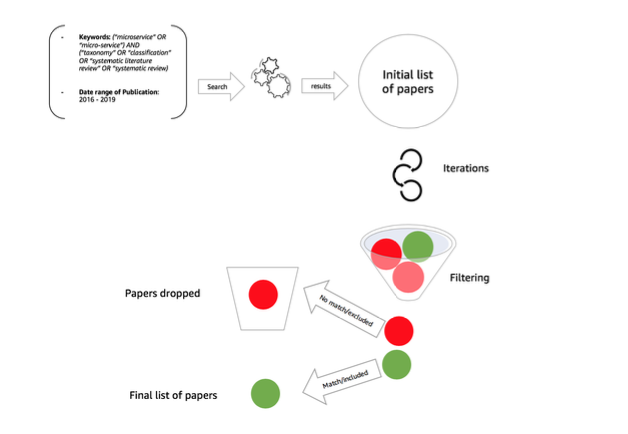
\includegraphics{searchstrategy.png}
\caption{Diagram of the search strategy.}
\end{figure}

\begin{table}[h!]
  \begin{center}
 \tiny
    \begin{tabular}{|l|l|l|l|} % <-- Alignments: 1st column left, 2nd middle and 3rd right, with vertical lines in between
    \hline
      1 & \makecell[l]{ Baresi et al. (2017) - Microservices Identification \\ Through Interface Analysis} & 11 & \makecell[l]{Masuda \& Viswanathan (2019) - Direction of \\ Digital IT and Enterprise Architecture}\\
      \hline
      2 & \makecell[l]{Jacopo Soldani et al. (2018) - The pains and gains of microservices: \\ A Systematic grey literature review} & 12 & \makecell[l]{Syed \& Fernandez (2018) - A reference architecture \\ for the container ecosystem}\\
      \hline
      3 & \makecell[l]{Vural et al. (2017) - A Systematic Literature \\ Review on Microservices} & 13 & \makecell[l]{Pahl \& Jamshidi (2016) - Microservices:  \\ A Systematic Mapping Study}\\
      \hline
      4 & \makecell[l]{Tetiana \& Anya (2018) - Overcoming Security Challenges \\ in Microservice Architectures} & 14 & \makecell[l]{Alshuqayran et al. (2016) - A Systematic Mapping Study \\ in Microservice Architecture}\\
      \hline
      5 & \makecell[l]{Marquez et al. (2018) - Review of Architectural Patterns and \\ Tactics for Microservices in Academic and Industrial Literature} & 15 & \makecell[l]{Taibi (2018) - Architectural Patterns for Microservices: \\ A Systematic Mapping Study}\\
      \hline
      6 & \makecell[l]{Rademacher et al. (2018) - Microservice architecture \\ and model-driven development} & 16 & \makecell[l]{Taherizadeh \& Stankovski (2017) - Auto-scaling Applications in \\ Edge Computing: Taxonomy and Challenges}\\
      \hline
      7 & \makecell[l]{Hamzehloui et al. (2019) - A Study on the Most Prominent \\ Areas of Research in Microservices} & 17 & \makecell[l]{Elsayed \& Zulkernine (2018) - A Taxonomy of \\ Security as a Service}\\
      \hline
      8 & \makecell[l]{Rademacher et al. (2018) - Towards a UML Profile for \\ Domain-Driven Design of Microservice Architectures} & 18 & \makecell[l]{Salah et al. (2016) - The evolution of distributed systems \\ towards microservices architecture}\\
      \hline
      9 & \makecell[l]{Garriga (2018) - Towards a Taxonomy of \\ Microservices Architectures} & 19 & \makecell[l]{Carvalho et al. (2019) - Greedy Multi-Cloud Selection Approach \\ to Deploy an Application Based on Microservices}\\
      \hline
      10 & \makecell[l]{Soldani et al. (2018). The pains and gains of microservices: \\ 
      A Systematic grey literature review} & 20 & \makecell[l]{Gill \& Buyya (2018) - Failure management for reliable \\ cloud computing: A taxonomy, model and future directions}\\
      \hline
    \end{tabular}
        \caption{List of papers included in the study}
    \label{tab:Table 1}
  \end{center}
\end{table}

The second sets of data that we relied on for this study was found by searching repositories for open source software. The two repositories that were selected for the study are Amazon Web Services (AWS) Serverless Application Repository (SAR) and GitHub. These two repositories were selected for a couple of reasons:

\begin{itemize} 


\item Their openness – although the AWS SAR is owned and managed by Amazon, the repository is opened for anyone to publish and use microservices 
\item Free of charge – both repositories can be used by anyone without any subscription or usage cost
\item Number and variety of microservices – A high number of microservices are published in both repositories (and GitHub in particular) more than any other publicly accessible repository. 

\end{itemize}


We started by running a generic search using the following keywords: (“microservices” OR “microservices architecture” OR “microservices composition”) AND (Publication date range 2016 – 2019). From this initial search, we used the first 300 results that matched our search criteria. This decision was based on the observation that lots of microservices were duplicated or there was no significant difference between the ones we excluded and the ones that were retained for the design of our taxonomy.

We then did some filtering based on the inclusion/exclusion criteria listed in the next section to further refine the results and narrow down the list to 100 microservices (full list in appendix) that were subjected to this study. Details of the criteria used for refining the results are provided in the next section.

\subsubsection{Sample of microservices selection}


\begin{itemize} 

\item \textbf{The first criterion} targets those microservices that have been utilized at least once as a component providing a functionality as part of a microservice-based application. Also considered falling into the same criteria are microservices that have already been used as part of a service composition process involving other microservices with a goal to provide a composed service. Service composition is process by which microservices are stitched together perhaps with or without some glue code (depending on their design and the target output application) in order to provide one or many functionalities. This process is believed to significantly reduces development time in that it helps leverage components that have already been built (Namoun et al., 2010).


\item \textbf{The second criterion} that was used to further refine our results was to select those microservices that could also be used as stand-alone to provide a given functionality in what could be referred to as single-microservice application. The rationale behind microservices as remark Dragoni et al. (2017) is to break down a monolithic application into small loose components that are independent from each other in terms of the technologies they are built on, how they are deployed and maintained. Microservices that do not provide a clear function when used in silo have been excluded as they were classified as being just an abstract piece of code that could only be used when associated with other pieces of code in the form of a microservice or perhaps only part of it. One of the advantages such capability provides is the opportunity to understand how microservices are deployed and whether or not they are only supported on certain platforms. In other words, it helps answer the question of whether the microservice is platform-dependent or whether it is platform-agnostic meaning it could be deployed on any platform.

\item \textbf{The third criterion} that we used was to only include only open source microservices that is those microservices that are free of charge, accessible to the general public and could be used as part of the development of microservices-based application. The main reason for excluding proprietary microservices is simply due to challenges around costs. Nonetheless, we still selected few proprietary ones to demonstrate that they are not significantly different to open source microservices as they appear to have more or less the same characteristics both functional and non-functional.

\item \textbf{The fourth criterion} that was used as part of the selection was the availability of the microservices accompanied by some documentation which contains at the very least the following information: the programming language, the deployment guide, platform supportability. Documentation is a key resource that helps gain an understanding of the microservice including detailed instructions on how it is deployed together with all the prerequisites that need to be met.

\item \textbf{The fifth criterion} that was used was to include only microservices that provided a clear functionality and to what extent it was flexible enough to be able to provide another functionality which is different from the one it was originally designed to deliver with no or very little design change.


\item \textbf{The sixth criterion} helped select microservices that were designed to interact with data in some way either as input, or to do some processing as part of some business logic or as output or all those options combined.


\item \textbf{The seventh criterion} that we used was to select based on the microservice or the resources in which the microservice was referenced was published. For that we only included those microservices resources that were published from 2016 and beyond. This was to ensure that no significant amount of time was wasted trying to understand some of the features of microservices that were potentially already outdated considering that the concept of microservice is a relatively new paradigm that is rapidly evolving especially with the speed of innovation that cloud computing introduces and microservices described to be very popular choice for designing cloud native applications (Sill, 2016). 

\end{itemize}

\subsection{Classification method}

To classify microservices we identify semantics from the users requirements for an application or service. Those semantics are keyword that can be used to describe the core functionality that a microservice provides and or the type technical action (such as analyzing log files, searching data, upload a file to name but a few) that is executed in the background. Once we have identified the semantics representing the functional classes of microservices, we then use a dimensional table to weight each non-functional attributes with a value between 0 and 5 with 5 being the highest weight indicating that a non-functional dimension is the most suitable for the functional class of microservice for which is it being weighted. The score of each functional class is calculated as per the math formula below based on the average score of each of the main non-functional dimensions namely Technology (excluding Data store), Deployment and Data store. We first calculate the total sum of the weighting for the all the dimensions and then we work out the average by dividing the total sum by the total number of dimensions. Once we have the average for each of the three dimensions, then we can easily calculate the overall average score for each functional dimension. The microservice will be classified under the functional class with the highest average score while the recommended technical dimensions would be the ones with the highest weight unless the user specifically states in the requirements their preference for a particular one.

Details of the formula used in the calculation shown below:

\[Score(functional)_{x}=\sum_{i=1}^{n}Xi \; \; \text{\textit{(Where X represents the weight and n the number of technical dimensions)}}\] 
\[(x \;is\; one\; of\; the \;3 \;non-functional \;dimensions\; group: \;Deployment,\; Technology \;and \;Data\; store) \]
%\[Average(functional)=\frac{\sum_{i=1}^{n}Xi}{total \; number \; of \; dimensions} \]

\[Average(functional)_{x}=\frac{Score(functional)_{x}}{total \; number \; of \; dimensions} \]

\[Average(functional)_{total}=\frac{\sum_{i=1}^{3}Score(functional)_{x}}{3} \]

\section{Taxonomy of microservices. A new framework}

\subsection{RQ1 - Functional attributes of microservices}

As shown in figure 2 below, the taxonomy is made of functional and non-functional dimensions. The boxes on the left side are the function types that basically serves for the classification of microservices. On the right side we have the non-functional dimensions which will be weighted to help determine which function(s) type(s) a microservice fits into. On the let side we have the functional dimensions that we believe microservices would typically fulfill. For instance, for microservices designed to fulfil a logging function, it is expected that the key component would be a data store and possibly flat files or some object store for storing log files, and as such those dimensions should carry the highest weight. In the next section we discuss both sets of dimensions (non-functional and functional) in more details. We have identify a total of 7 main functional attributes which are listed below:

\begin{figure}[h!]
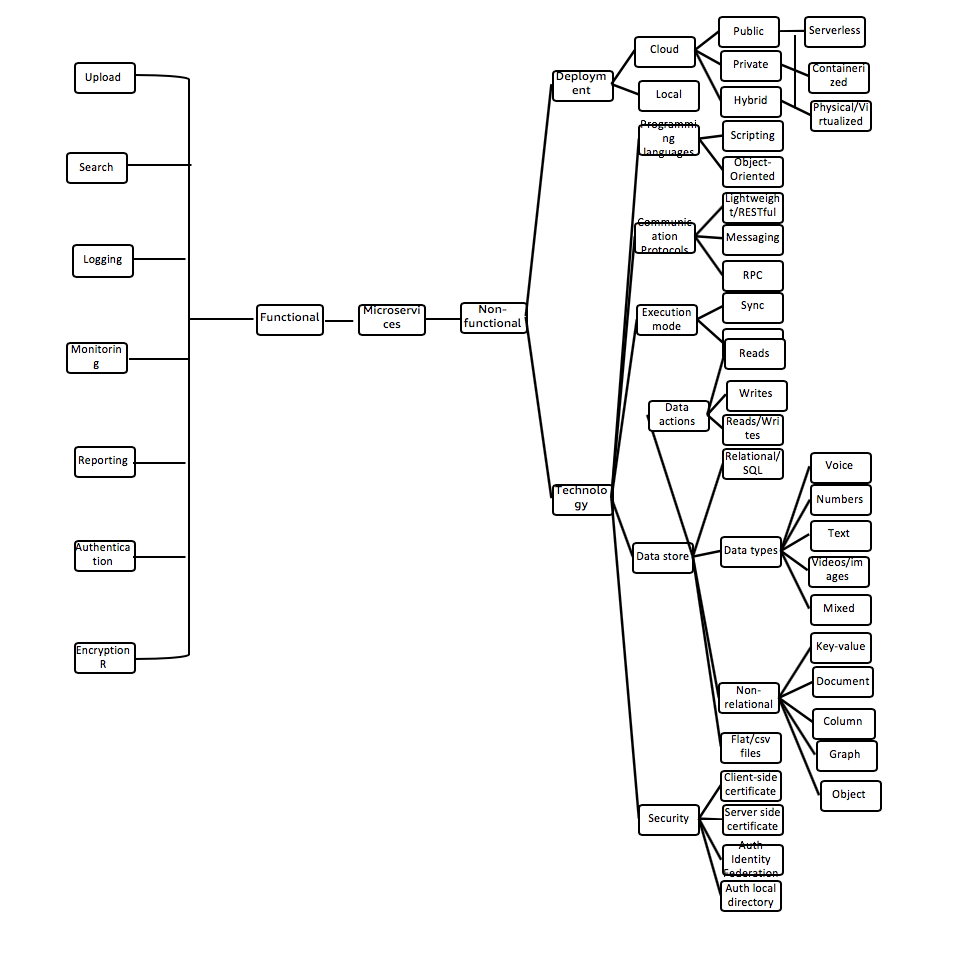
\includegraphics{taxonomydiagram.png}
\caption{Taxonomy of Microservices.}
\end{figure}

\begin{itemize}
\item \textbf{Encryption}
This functional security characteristic is attributed to any microservice that is specifically designed to provide data security functionality such as encryption of data at rest or in transit. Anoter example are those microservices that are used as part of an application or a service to provide encryption of security keys. 

\item \textbf{Authentication}
This is another functional security attribute that identifiy those microservices that are designed to handle identity and access for users or applications. Some examples of such services are Amazon Identity and Access Management (IDM), Amazon Cognito user pools or Microsoft Azure AD provide such functionalies.

\item \textbf{Reporting}

The reporting attribute characterise those microservices that are designed to read historical data from a data store and display to some kind of presentation layer. Such functionality could be provided by a dedicated microservice or as part of a composed microservice-based application. Microservices providing reporting function would typically work with data store which could be provided that another microservice.

\item \textbf{Monitoring} 

Monitoring is about checking the state of a component which could be a hardware or software component. The monitoring could be done on individual part of an application or on the entire application. Any microservice that react (sending an alert, orchestrate a remediation script, etc.) to a change of state of an application component is deemed to have a monitoring functional attribute.

\item \textbf{Logging}

Microservices that are design to fulfill log management function would have this attribute. This attribute can be closely related to monitoring as monitoring can be done by analyzing logs to find root cause of problem.

\item \textbf{Search}

The search function is for any microservice that performs some kind of search which means it would require a data store from where to search for data. An example of is Amazon Elasticsearch.

\item \textbf{Upload}

Upload functional attribute is for those microservices that manipulate files and more specifically upload files into a repository. Service like as Amazon secure file transfer (SFTP) is a good example of service with this attribute.

\item \textbf{Other}

While we expect most microservice functions to fall into one of the category mentioned above, there are other functions that may also be looked as separate attribute. Those microservices fall under the category other . A good example of that is industry specific domain such as fintech, retail or media and entertainment to name just a few.

\end{itemize}

\subsection{RQ2 - Mapping of functional to technical attributes of microservices}

This research proposes a new framework that allows for a more fine-grained taxonomy of microservices. Previous work done by Garriga (2018) have shown some limitations in classifying web services. To demonstrate how functional attributes of microservices map to technical ones we use an example of microservice-based application.

\begin{figure}[h!]
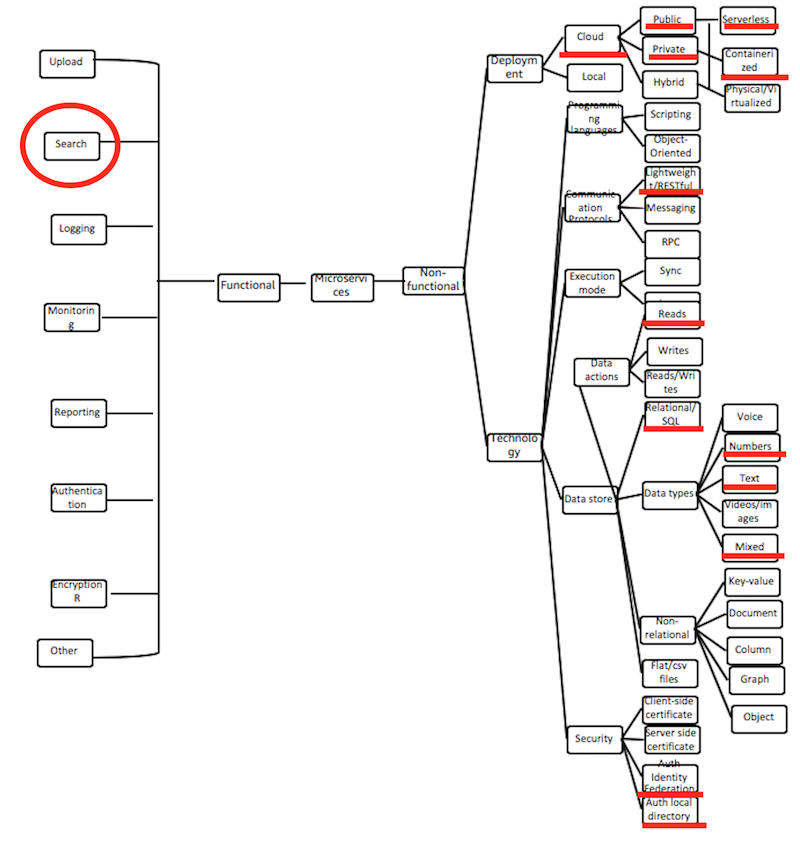
\includegraphics{func2techmapping.png}
\caption{Mapping of non-functional to functional attributes of Microservices.}
\end{figure}


\textbf{- Meeting room status reporting example}

Let's look at the example of a meeting room reporting application that provides a real time report of all the meeting rooms that have been booked but which are not utilized. How could one go about retrieving discrete microservices components that make of the overall microservice to provide the sought functionality?

In this framework we propose using the keywords and map them to specifics function. In the case of the example above we have “real time report” will be mapped to reporting functionality while “all the meeting rooms” will indicate some sort of “querying” functionality. We also have “booked but not utilized” which corresponds to a state would most likely map to a “monitoring” functionality. last but not least the keywords “meeting room” that in itself could constitute a function such as a microservice for meeting rooms management. See table 2 below for details of full mapping.


\begin{table}[h!]
  \begin{center}
  \small
    \begin{tabular}{|l|l|} % <-- Alignments: 1st column left, 2nd middle and 3rd right, with vertical lines in between
    \hline
    \textbf{Keyword} & \textbf{Function}\\
    \hline
      \multirow{3}{*}{Looking for} & Search\\
      & Monitoring\\ 
      & Ingestion\\
      \hline
      Real time & Monitoring/Reporting\\
      \hline
      Report & Display/Reporting\\
      \hline
      Meeting rooms & Meeting rooms management\\
      \hline
      Booked/Not utilized & Monitoring/Search/meeting rooms management\\
      \hline
    \end{tabular}
        \caption{Keywords-to-function mapping table example}
    \label{tab:Table 2}
  \end{center}
\end{table}


When we analysed microservices selected for this study it is possible that each one provides a completely different function as part of a microservice-based application. However, most of these functions could be group into the following family of functions:

\begin{itemize}


\item Search
\item Monitoring
\item Logging
\item Authentication
\item Encryption
\item Compression
\item Reporting
\item Data ingestion
\item Upload
\end{itemize}

As shown in figure 3 above, the microservices under our taxonomy is classified under the search functionality identified with the red circle. On the right hand side we can also see the non-functional attributes that best fit the requirements of the meeting room status reporting example. For instance, we can see that the best database choice would be a relational database type while the best communication protocols that best address the best aligns with the requirements of a Search function microservice type is lightweight Restful protocol. In section 7 we discuss in details how the mapping process is done using mathematical formula.

\subsection{RQ3 - Classifying and selecting microservices}

This approach of classifying microservices by function aligns very much with Newman (2015) when he talks about focusing service boundaries on business boundaries to help identify code that provide a given piece of functionality. Looking at microservices from a business function lens would help non-technical readers not only understand microservices from a non-technical standpoint, but also provide that with enough ground to get involve and contribute in the decision process for microservices adoption within the enterprise. Equally, scholars and researchers that may want to conduct research on microservices in business field would have an interest in this approach of classifying microservices.

Dragoni et al. (2017) define microservices from technical point of view as independent components conceptually deployed in isolation and equipped with dedicated memory persistence tools (e.g. databases). They argue that since all the components of a microservice architecture are microservices, its distinguishing behaviour derives from the composition and coordination of its components via messages. This indicates that microservices could be classified by the technical attributes of their components. By following that approach, this framework uses technology-related attributes as second type of dimensions for identifying microservices. And that is where our research and the study conducted previously by Garriga (2018) align. Microservices can therefore be classified say based on the programming languages used for their development e.g. scripting, object-oriented, etc. Their communication protocols such as Restful/http(s), MQ, xml, etc. The data store including relational databases, NoSQL databases. The other technical dimensions are data transfer methods (push/pull, sync/async, streaming); the platforms and the deployment method. Table 3 below shows the technical dimensions that we identified as possible options for classifying microservices.

\begin{table}[h!]
  \begin{center}
  \tiny
    \begin{tabular}{|l|l|l|l|l|l|l|} % <-- Alignments: 1st column left, 2nd middle and 3rd right, with vertical lines in between
    \hline
    \textbf{\makecell[l]{Programming \\ Languages}} & \textbf{Communication} & \textbf{\makecell[l]{Data \\ store}} & \textbf{\makecell[l]{Data \\ transfer}} & \textbf{Platform} & \textbf{OS} & \textbf{Deployment}\\
      \hline
      \makecell[l]{Scripting \\ Object-oriented \\ Procedural \\ Other} & \makecell[l]{Restful/http \\ MQ \\ RPC \\ XML} & \makecell[l]{Relational DB \\ NoSQL DB \\ Graph \\ Object \\ Flat files} & \makecell[l]{Push \\ Pull \\ Synch \\ Asynch \\ Streaming} & \makecell[l]{Virtual machines \\ Physical servers \\ Containers \\ Serverless} & \makecell[l]{Windows \\ Linux \\ Other} & \makecell[l]{Public cloud\\ Private cloud \\ On-premise \\ Hybrid}\\
      \hline
    \end{tabular}
        \caption{Microservices technical dimensions}
    \label{tab:Table 3}
  \end{center}
\end{table}

In table 4 below we zoom in on programming languages and data types dimensions, and we see that it is possible to further classify microservices by programming language sub-dimensions including Python, JavaScript, PHP, Go, Ruby, html, C\#, Java and the type of data being manipulated such as text, video or voice.

\begin{table}[h!]
  \begin{center}
    \begin{tabular}{|l|l|} % <-- Alignments: 1st column left, 2nd middle and 3rd right, with vertical lines in between
    \hline
    \textbf{\makecell[l]{Programming \\ language}} & \textbf{Data type}\\
      \hline
      \makecell[l]{Python \\ Javascript \\ Java \\ PHP \\ Go \\ HTML \\ C\#} & \makecell[l]{Text \\ Numbers \\ Videos \\ Images \\ Voice \\ Mixed \\ Other} \\     
       \hline
    \end{tabular}
        \caption{Programming languages \& Data types}
    \label{tab:Table 4}
  \end{center}
\end{table}

The other dimensions the framework looks at are the dependencies as well as compatibilities, in other words what are the microservices that would require one or more other microservices in order to fulfil a given function (dependency) or are there some microservices that cannot work together for one reason or another (compatibility).

\subsubsection{Non-functional dimensions}

\begin{itemize}

\item \textbf{Deployment}


This dimension indicates whether the microservices can be deployed and run on a server located in a data centre on-premise refer to as “local” in the diagram. Or whether, the microservices needs to be run in the cloud which is further subdivided into private, public and hybrid type. Also, for the deployment dimension, microservices could be further classified based on the type of compute service used to run them including physical, virtual machine or inside a container such as docker or kubernetes, or in a dynamically powered server by an event also known as serverless.

\item \textbf{Technology}

From a technology standpoint, microservices can be classified based on the type of programming language that they are developed on. For instance, Java-based or C++ microservices for object-oriented types, JavaScript for scripting language and so on. 

The second sub-dimension under technology is the communicating protocols used for when communicating with other microservices. A lightweight API gateway based on HTTP/RESTful could be used or a message transfer protocol such as MQ could be used as its name implies for transferring messages between microservices. The other option might be a remote procedure call whereby a microservice would trigger the execution of a function call on a remote server.

The next sub-dimension under technology is whether the execution done synchronously or asynchronously. This subdimension is somewhat tightly related to the communication protocols and are sometime used interchangeably. In reality they designate two distinct concepts albeit the close relation between those concepts. In general, messaging queuing tend to be more suitable for asynchronous execution type whereas synchronous execution mode tends to work with lightweight protocols such as REST but that is not always the case.

The other type of dimension type of technology subdimension is the data store. Microservices could be designed to use relational, non-relational data store or even flat files for storing data. Relational data stores are more suitable for microservices that are expected to manipulate structured data and such data could be accessed using standard SQL queries. Some microservices are designed to work with non-relational data store in order to address specific use cases that require handling unstructured data, and for that various options are available including key-value, document or graph databases which typically can store larger amount of data than relational databases as noted by Vicknair (2010). Another option for non-relational database are object storage type such as amazon s3 typically used for data lake given the amount of data it can store. Data could also be stored in files such as csv or text files although this method is less and less utilized perhaps due to the variety of databases for structured and unstructured data available today as open source and also the continued drop in price of the COTS (Commercial-Off-The-Shelf) ones.

Another key technology dimension for microservices is the type of data that is processed by the microservices and this include input and output data which could be in the form of texts, numbers, voice (such as amazon Alexa or google assistant), videos or images or in some cases a combination of two or more data types which we classify in the taxonomy as mixed data type.

The other technology dimension that the framework proposes using for classifying microservices is security and for that we’ve identified four categories including microservices using client side certificates and the ones using server side certificates on one hand, and on the other hand microservices using some kind of local directory such as Microsoft Active directory or LDAP to authenticate users or applications and microservices using identify federation for authenticating users which could be based on technologies such as SAML, OAuth or OpenID.

\end{itemize}
\section{Description of the taxonomy}


In our framework microservices are classified based on two main dimensions that is functional and non-functional dimensions. For a fine-grained classification we use a weighting mechanism of non-functional dimensions to be able to classify microservices by type of functionality to functionalities they are designed to provide e.g. Logging, Authentication. The weighting ranges from between 0 and 5 with zero being the lowest weight meaning that any dimension with a weight of zero has very little or no influence in the classification by functionality of the microservice. The deployment dimension carries the lowest weight while a weighting of 5 means the dimension carries the highest weight which indicates that the dimension is the most important one in helping classifying microservices with that particular dimension. For example, an authentication microservice will have a weight of 1 for the deployment dimension for most microservices tend to be platform-agnostic given that they can run both on premise and in the cloud either by installing them directly on a server instance or by deploying inside a container. Exception to that is if it is specifically stated in the requirements that a particular deployment method is preferred in which case the weighting should be 5 (the highest). Figure 3 below shows how weighting is applied to non-functional dimensions.

\begin{figure}[h!]
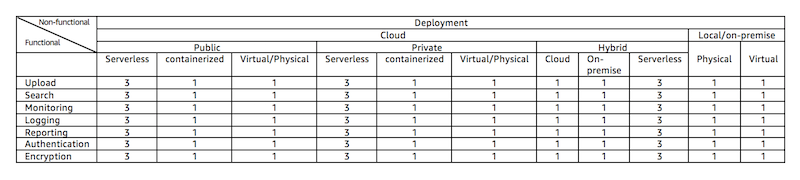
\includegraphics{table5.png}
\caption{Weighting of non-functional dimensions: Deployment.}
\end{figure}

From figure 3 above we can see that the most influential dimension for classifying microservices from a deployment perspective is the serverless characteristic which can be implemented in the cloud (public, private). Serverless is a relatively new concept that allows running an application piece of code without the need to operate or manage the server that it is deployed on. It is an approach which Castro (2017) qualifies as function as a service that makes life easier for the developer who only has to write the code and not worry about the underlying infrastructure. The dynamic nature of cloud makes it a good platform for serverless-based microservices. 

\begin{figure}[h!]
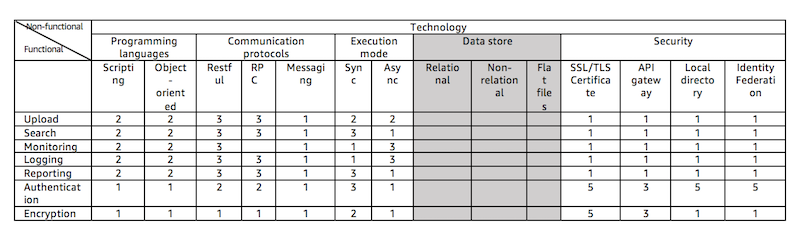
\includegraphics{table6.png}
\caption{Weighting of non-functional dimensions: Technology}
\end{figure}

If we take a look at the technology dimensions we can see from figure 4 above that Upload type of microservices would mostly use RESTful or RPC communication protocol type while they could execute synchronously or asynchronously. Zimmermann (2017) cites RESTful HTTP as one of the most widely used communication protocol for microservices designed to help overcome the limitations of Service Oriented Architecture (SOA). The rest of the dimensions have very little influence in terms of where to classify the microservice hence their weighting of 1 except for the programming language that has a weight of 2 but still does not differentiate the microservice as both language types (scripting and object-oriented) carry an equal weight of 2. It is pretty obvious that microservices providing security functionality such as authentication and encryption have the highest weight on SSL/TLS certificate, API gateway, local directory and identity federation dimensions.

\begin{figure}[h!]
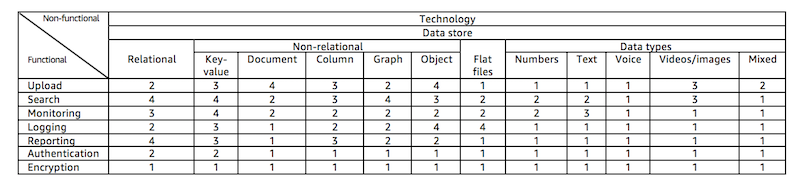
\includegraphics{table7.png}
\caption{Weighting of non-functional dimensions: Technology/Data Store}
\end{figure}

In the Figure 5 above, we zoom into the data store dimension and we can see that microservices that use relational database in general would fall into the group of microservices providing search or reporting function while the logging functionality is mostly provided by microservices that are designed to work with flat files or object storage as data store. 

Now let us use the data in figure 3, 4 and 5 above to replace the variables in our math formula to see what result we get:

\[Score(Upload)_{deployment}=\sum_{i=1}^{11}Xi = 17\] 
\[Score(Upload)_{technology}=\sum_{i=1}^{11}Xi = 19\] 
\[Score(Upload)_{ds}=\sum_{i=1}^{12}Xi = 27\] 
\[Average(Upload)_{deployment}=\frac{17}{11} = 1.54 \]
\[Average(Upload)_{technology}=\frac{19}{11} = 1.72 \]
\[Average(Upload)_{ds}=\frac{27}{12} = 2.25 \]
\[Average(Upload)_{total}=\frac{1.54 + 1.72 + 2.25}{3} = 1.83\]

In the same way we can calculate the average score for the the functional attributes:

\[Average(Upload)_{total}=\frac{1.54 + 1.72 + 2.25}{3} = 1.83\]
\[Average(Search)_{total}=\frac{1.54 + 1.72 + 2.58}{3} = 1.94\]
\[Average(Monitoring)_{total}=\frac{1.54 + 1.45 + 2.27}{3} = 1.75\]
\[Average(Logging)_{total}=\frac{1.54 + 1.45 + 1.91}{3} = 1.63\]
\[Average(Reporting)_{total}=\frac{1.54 + 1.45 + 1.75}{3} = 1.58\]
\[Average(Authentication)_{total}=\frac{1.54 + 2.63 + 1.16}{3} = 1.77\]
\[Average(Encryption)_{total}=\frac{1.54 + 1.63 + 1}{3} = 1.39\]

From the above calculation we can classify the microservice into the category of Search function as it has the highest average score of 1.94

\section{Classification of microservice example using the taxonomy}

If we take as an example a microservice from our sample: microservice-http-endpoint that we found on Amazon Web Services (AWS) serverless Application Repository (SAR) with the code available in awslabs GitHub repository \url{https://github.com/awslabs/serverless-application-model/tree/master/examples/apps/microservice-http-endpoint}.

It is a basic microservice that performs a read and write to and from a non-relational database via a Restful API using amazon API gateway. This microservice is serverless by design as it does not require having to deploy or manage any server for running it, instead it’s been developed in such a way that all the infrastructure resources that it requires (in this case some Amazon cloud services) are referenced in the form of code within a template file written in yaml or json format. These infrastructure resources will be spun up when the code runs which effectively means when the microservice is invoked. Let’s try to understand the most important parts of the contents from template file below:

AWSTemplateFormatVersion: '2010-09-09'
Transform: 'AWS::Serverless-2016-10-31'
Description: >-
  A simple backend (read/write to DynamoDB) with a RESTful API endpoint using Amazon API Gateway.
Parameters: 
  TableNameParameter: 
    Type: String
Resources:
  microservicehttpendpoint:
    Type: 'AWS::Serverless::Function'
    Properties:
      Handler: index.handler
      Runtime: nodejs6.10
      CodeUri: .
      Description: >-
        A simple backend (read/write to DynamoDB) with a RESTful API endpoint using Amazon API Gateway.
      MemorySize: 512
      Timeout: 10
      Policies:
        - DynamoDBCrudPolicy:
            TableName: !Ref TableNameParameter
      Events:
        Api1:
          Type: Api
          Properties:
            Path: /MyResource
            Method: ANY

The line of code Transform: 'AWS::Serverless-2016-10-31' tells the interpreter that this is a serverless microservices which contains a number of resources that will be deployed as code as with the microservice. Those resources are specified under Resources section. We can see that a lambda function - which is a compute service from Amazon Web Services that let you run your code without provisioning or managing servers – is listed as resource using the following line of code:  
Type: 'AWS::Serverless::Function'. The code for this particular lambda function is written in nodejs6.10 which is precisely what the following line of code does Runtime: nodejs6.10. The other resources are DynamoDB which is amazon managed non-relational database service and an API gateway, a managed API gateway service. The codes for both resources are shown below:

        - DynamoDBCrudPolicy:
            TableName: !Ref TableNameParameter
      Events:
        Api1:
          Type: Api
          Properties:
            Path: /MyResource
            Method: ANY

We can see that this microservice is heavily tied to a cloud platform and it can only be deployed without being modified to Amazon cloud. Also, the microservice is of serverless type which explains why the serverless on cloud dimension would carry more weight from a deployment perspective if we were to classify this microservice. From a communication protocol perspective, the microservice is making Restful api calls as indicated in the code. As there is no data to tell whether the microservice execute synchronously or asynchronously nor any indication on the security technology used if any we will give those dimensions a weight of 0. This leaves us with the data store dimension to finalize our classification. The microservice uses DynamoDB which is a key-value data store which at this point makes it falls under a Search or Monitoring type of microservice. However, we will look further into the type of database action this eliminates the possibility of this microservice being classify as Search type, for search tend to perform read only action. This effectively means that the microservice-http-endpoint having scored high on serverless (no server to deploy/manage), cloud (Amazon public cloud), Restful api call, key-value data store (Amazon DynamoDB) with read and write database actions will highly likely performing a monitoring function hence fall into the Monitoring category of microservice.

\section{Limitations}

While we have demonstrated that the methodology used in this research has led to the design of our new taxonomy for microservices, it goes without saying that it has its shortcomings. In this section we discuss the limitations of our method.

\begin{itemize}


\item \textbf{A very large number of microservices}

One of these limitations stems from the sheer number of microservices that are available today, a number that keeps on increasing every day as new microservices are being built by software developers. That begs the question as to whether the sample we selected for this study is representative enough of all the microservices that are available in the industry today. While we feel that our method was rigorous enough to account for all possibilities in terms of microservices attributes (common and specifics), we cannot exclude totally the possibility of us missing out on some which perhaps could have led to slightly different results. 

\item \textbf{No access to proprietary or private microservices}

In our study we did not include microservices that are proprietary and that are not publicly accessible. While we expect such microservices to share some common attributes with those that are made available to the general public, we have no knowledge of their specifics in terms of which technologies they are designed with, how they are deployed, what functions they fulfil and whether or not they can run on any environment. All these questions are very interesting ones that perhaps would need exploring as part of a new study.

\item \textbf{Too many technology options}

This one is more of a challenge than a limitation to our study. One of the advantages of microservices is their flexibility in terms of the freedom developers have to choose which programming language they want to use when building microservices. Dragoni et al. (2017) acknowledge the value that microservices bring with such flexibility as it provides users with more options to choose from and more flexibility in terms of the technology they can use to build applications. Singleton (2106) also discuss in his paper “The economics of microservices” talks about the flexibility that software engineers have in choosing the technology they want for building microservice-based applications acknowledging that it does provide a number of advantages including reducing the costs of developing and maintaining software while increasing the speed at which software can be released. The downside of that which proved to be a real challenge in our study is that trying to classify microservices by technology dimensions is very cumbersome with so many options to choose from given the plethora of technologies that is available in the industry today. If we take for instance programming languages, trying to classify microservices by programming languages, could easily lead to several hundreds of options. And even by trying to group them into family of programming languages, that is languages that use the same approaches such as object-oriented, scripting or procedural languages type to name but a few we would still end up with several options. 

\item \textbf{The precision and efficiency of our search strategy}

The keywords for searching our target microservices as well as the repositories and libraries searched should have enabled us to cover a broader scope. While we looked into the most popular academic and scientific libraries and journals, there is possibility that we missed a completely different type of microservices such as microservices that are not indexed with our chosen keywork which potentially could have produced different results. There is also a question mark on whether we were able to capture all the functional characteristics especially with domain specific microservices such as the one providing Artificial Intelligence, IoT or Blockchain functions or even tailored to specific industry such as healthcare, financial or retail. If we take look at microservices functions from a perspective of possible HTTP methods that can be used by web services it becomes obvious that the DELETE method has not been accounted for which may indicate that we might have missed other functions with our method.

Despite the aforementioned limitation we still feel that our taxonomy represents a good foundation for classifying and selecting microservices. That being said further work could be undertaken to either fine-tune our taxonomy or provide a much granular one. In the next section we look into the opportunities for further work.

\end{itemize}

\section{Summary and future work}


In this paper we look at the existing taxonomy of microservices and how they can be used to classify microservices. Next, we discussed the limitations of the existing taxonomy which introduced us to the newly proposed framework. We explained how microservices could be classified by function they provide based on the technology dimensions. Each dimension is assigned a weighting which basically is a number between 0 and 5, with 0 representing the lowest measurement which indicates that the dimension has little or no influence over the classification of the microservice, while 5 is an indication that a dimension is the most important in helping determine which type of function the microservice delivers hence should be classify as. We discussed the different dimensions that can be used which are technology and deployment related dimensions. The deployment dimensions were subdivided into Cloud and local/on-premise which were further divided into 10 subdimensions including private, public, hybrid cloud, virtual/physical, container, serverless to name but a few. The technology dimensions were identified as the key ones for helping classify microservices under our taxonomy and they include programming languages, communication protocols, execution mode, security, data stores, data types, database actions and more. To test the taxonomy, we then used an example of microservice taken randomly from amazon serverless repository and walked through the process of classifying microservice using our framework. 

While this taxonomy could be regarded as a significant step forward for helping classify microservices, more work can still be done to improve the taxonomy. For instance, we could look at the code level to try to identify common patterns that microservices share which eventually could be accounted for in their classification. We could also look at things like frameworks, packages and libraries that can help identify microservices. Another dimension that could be looked at is the compatibility of microservices in other words look at a way of classifying microservices based on their ability to work with each other to provide one of more functions. Another research that could be done building on the finding of the study is to look into designing a framework for discovering microservices which would appear like a logical evolution from of a taxonomy for classifying microservices.

\pagebreak 
\section{References}

\begin{enumerate}

\item Andrews, B. and Kumar Ramesh, S. (2019). awslabs/serverless-application-model. [online] microservice-http-endpoint. Available at: https://github.com/awslabs/serverless-application-model/tree/master/examples/apps/microservice-http-endpoint [Accessed 15 May 2019].


\item Alshuqayran, N., Ali, N., \& Evans, R. (2016). A Systematic Mapping Study in Microservice Architecture. 2016 IEEE 9th International Conference on Service-Oriented Computing and Applications (SOCA). 



\item Baresi, L., Garriga, M., \& Renzis, A. D. (2017). Microservices Identification Through Interface Analysis. Service-Oriented and Cloud Computing Lecture Notes in Computer Science,19-33.



\item Castro, P., Ishakian, V., Muthusamy, V., \& Slominski, A. (2017). Serverless Programming (Function as a Service). 2017 IEEE 37th International Conference on Distributed Computing Systems (ICDCS). 


\item Chen, L. (2018). Microservices: Architecting for Continuous Delivery and DevOps. 2018 IEEE International Conference on Software Architecture (ICSA). 


\item Dmitry Namiot, Manfred Sneps-Sneppe (2014). On Micro-services Architecture. International Journal of Open Information Technologies ISSN: 2307-8162 vol. 2, no.9, 2014


\item Dragoni N. et al. (2017) Microservices: Yesterday, Today, and Tomorrow. In: Mazzara M., Meyer B. (eds) Present and Ulterior Software Engineering. Springer, Cham.


\item Elsayed, M., \& Zulkernine, M. (2018). A Taxonomy of Security as a Service. Lecture Notes in Computer Science On the Move to Meaningful Internet Systems. OTM 2018 Conferences, 305-312. 


\item F., Márquez, G., \& Astudillo, H. (2018). Exploration of academic and industrial evidence about architectural tactics and patterns in microservices. Proceedings of the 40th International Conference on Software Engineering Companion Proceeedings - ICSE 18. 


\item Garriga M. (2018) Towards a Taxonomy of Microservices Architectures. In: Cerone A., Roveri M. (eds) Software Engineering and Formal Methods. SEFM 2017. Lecture Notes in Computer Science, vol 10729. Springer, Cham


\item Hamzehloui, M. S., Sahibuddin, S., \& Ashabi, A. (2019). A Study on the Most Prominent Areas of Research in Microservices. International Journal of Machine Learning and Computing, 9(2), 242-247. 


\item J., Vieira, D., \& Trinta, F. (2019). Greedy Multi-Cloud Selection Approach to Deploy an Application Based on Microservices. 2019 27th Euromicro International Conference on Parallel, Distributed and Network-Based Processing (PDP). 


\item Masuda, Y., \& Viswanathan, M. (2019). Direction of Digital IT and Enterprise Architecture. Enterprise Architecture for Global Companies in a Digital IT Era, 17-59. 


\item Namoun A., Wajid U., Mehandjiev N. (2010) Service Composition for Everyone: A Study of Risks and Benefits. In: Dan A., Gittler F., Toumani F. (eds) Service-Oriented Computing. ICSOC/ServiceWave 2009 Workshops. ServiceWave 2009, ICSOC 2009. Lecture Notes in Computer Science, vol 6275. Springer, Berlin, Heidelberg


Pahl, C., \& Jamshidi, P. (2016). Microservices: A Systematic Mapping Study. Proceedings of the 6th International Conference on Cloud Computing and Services Science. 


\item Rademacher, F., Sorgalla, J., Wizenty, P. N., Sachweh, S., \& Zündorf, A. (2018). Microservice architecture and model-driven development. Proceedings of the 19th International Conference on Agile Software Development Companion - XP 18. doi:10.1145/3234152.3234193


\item Rademacher, F., Sachweh, S., \& Zündorf, A. (2018). Towards a UML Profile for Domain-Driven Design of Microservice Architectures. Software Engineering and Formal Methods Lecture Notes in Computer Science, 230-245. 


\item S. Newman (February 2015), Building Microservices: Designing Fine-Grained Systems, O'Reilly Media, 1st edition


\item S. S., \& Buyya, R. (2018). Failure Management for Reliable Cloud Computing: A Taxonomy, Model and Future Directions. Computing in Science \& Engineering, 1-1. doi:10.1109/mcse.2018.2873866


\item Salah, T., Zemerly, M. J., Yeun, C. Y., Al-Qutayri, M., \& Al-Hammadi, Y. (2016). The evolution of distributed systems towards microservices architecture. 2016 11th International Conference for Internet Technology and Secured Transactions (ICITST). 

\item Sill, A. (2016). The Design and Architecture of Microservices. IEEE Cloud Computing, 3(5), 76-80. 


\item Singleton, A. (2016). The Economics of Microservices. IEEE Cloud Computing,3(5), 16-20


\item Soldani, J., Tamburri, D. A., \& Heuvel, W. V. (2018). The pains and gains of microservices: A Systematic grey literature review. Journal of Systems and Software,146, 215-232


\item Syed, M. H., \& Fernandez, E. B. (2018). A reference architecture for the container ecosystem. Proceedings of the 13th International Conference on Availability, Reliability and Security - ARES 2018. 


\item Taibi, D., Lenarduzzi, V., \& Pahl, C. (2018). Architectural Patterns for Microservices: A Systematic Mapping Study. Proceedings of the 8th International Conference on Cloud Computing and Services Science. 


\item Taherizadeh, S., \& Stankovski, V. (2017). Auto-scaling Applications in Edge Computing. Proceedings of the International Conference on Big Data and Internet of Thing - BDIOT2017. 


\item Vicknair, C., Macias, M., Zhao, Z., Nan, X., Chen, Y., \& Wilkins, D. (2010). A comparison of a graph database and a relational database. Proceedings of the 48th Annual Southeast Regional Conference on - ACM SE 10. 


\item Vural, H., Koyuncu, M., \& Guney, S. (2017). A Systematic Literature Review on Microservices. Computational Science and Its Applications – ICCSA 2017 Lecture Notes in Computer Science, 203-217. 


\item Yarygina, T., \& Bagge, A. H. (2018). Overcoming Security Challenges in Microservice Architectures. 2018 IEEE Symposium on Service-Oriented System Engineering (SOSE). 


\item Zimmermann, O. Computer Science Research \& Development (2017) 32: 301. \url{https://doi.org/10.1007/s00450-016-0337-0} 

\end{enumerate}


\end{document}
 